\documentclass{article}
\usepackage[T1]{fontenc}
\usepackage{lmodern}
\usepackage{graphicx}
\usepackage{amsmath,amssymb}
\usepackage[a4paper,margin=2cm]{geometry}
\usepackage[absolute,overlay]{textpos}
\setlength{\TPHorizModule}{1mm}
\setlength{\TPVertModule}{1mm}
\usepackage[indonesian]{babel}
\usepackage{hyperref}
\setlength{\emergencystretch}{2em}
% unit: Halaman 18

\begin{document}

% === Halaman 18 (llm) ===

\vspace{89.40mm}

\section*{Perfect Secrecy}

\begin{itemize}
    \item \textit{Perfect secrecy}: Cipherteks tidak menyediakan informasi apapun tentang plainteks maupun kunci.
    \item Pada tahun 1949, Claude Shannon dari Laboratorium Bell membuktikan bahwa OTP memiliki \textit{perfect secrecy}. Ia menulis pembuktian tsb di dalam makalahnya:
    
    \textcolor{red}{"Shannon, C. E. (1949). Communication theory of secrecy systems. Bell System Technical Journal, 28(4), 656--715."}
    
    \item Menurut Shannon, suatu sistem memiliki \textit{perfect secrecy} apabila setelah penyerang memperoleh cipherteks, informasi mengenai plainteks tidak bertambah. Secara matematis, kondisi tersebut dinyatakan sebagai:
    
    \[ P(P = p \mid C = c) = P(P = p) \]
    
    Artinya, probabilitas suatu plainteks tertentu tetap sama sebelum maupun setelah cipherteks diamati
\end{itemize}

% deskripsi: Foto potret Claude Shannon
% bbox normalisasi: [0.8580, 0.0240, 0.9760, 0.3250]
\begin{textblock*}{24.78mm}(180.18mm,7.13mm)
\noindent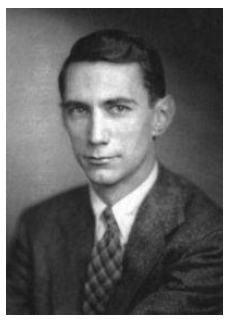
\includegraphics[width=24.78mm,height=89.40mm]{../../images/llm/page_018_img_01.png}%
\end{textblock*}

\end{document}
